\documentclass[preprint]{sigplanconf} % <<<

\usepackage{amsmath}
\usepackage{amssymb}
\usepackage{amsthm}
\usepackage{graphics}
\usepackage[latin1]{inputenc}
\usepackage{microtype}  % do not remove
\usepackage{pygmentize}
\usepackage{rgalg}
\usepackage{tikz}
\usepackage{xcolor}
\usepackage{xspace}

\usepackage[colorlinks]{hyperref} % keep it last to avoid some warnings

\RecustomVerbatimEnvironment{Verbatim}{BVerbatim}{}
\definecolor{darkred}{rgb}{0.4,0,0}
\definecolor{darkblue}{rgb}{0,0,0.4}
\definecolor{verylightgray}{rgb}{0.9,0.9,0.9}
\definecolor{lightblue}{rgb}{0,0,0.9}
% comment the next line for printing
\hypersetup{colorlinks,linkcolor=darkblue,citecolor=darkblue,urlcolor=darkblue}
\hypersetup{
  pdftitle={A Language for Specifying Safety Temporal Properties of Object-Oriented Programs},
  pdfauthor={Radu Grigore and Rasmus Lerchedahl Petersen and Dino Distefano}}

\newcommand{\TPL}{TOPL}

\titlebanner{DRAFT}
\title{\TPL: A Language for Specifying Safety Temporal Properties of Object-Oriented Programs}
\authorinfo{Radu Grigore \and Rasmus Lerchedahl Petersen \and Dino Distefano}{Queen Mary, University of London}{{\rm\{}rgrig,rusmus,ddino{\rm\}}@eecs.qmul.ac.uk}

% rg: I tend to give grammars in BFS order
\def\grammar#1{{
  \footnotesize
  \def\b##1{{\rm\Verb@##1@}}\def\*{$^*$}\def\?{$^?$}\def\({$($}\def\){$)$}
  \def\|{$\mid$}\def\+{$^+$}
  \smallskip
  \hbox to\hsize{\hfil\vbox{\halign{\hfil\it##&$\;::=\;$\it##\hfil&\qquad\rm##\hfil\cr#1}}\hfil}
  \smallskip
}}

\renewcommand{\sectionautorefname}{Section}
\renewcommand{\subsectionautorefname}{\sectionautorefname}

\newcommand{\note}[2]{\textcolor{gray}{[\textcolor{red}{#1}: #2]}}
\newcommand{\rg}[1]{\note{rg}{#1}}
\newcommand{\rlp}[1]{\note{rlp}{#1}}
\newcommand{\dd}[1]{\note{dd}{#1}}
\newcommand{\dinocomment}[1]{\dd{#1}}

\newcommand{\N}{\ensuremath{\mathbb{N}}}
\newcommand{\delimitVerbatim}{\par\nobreak\smallskip\noindent}
\newcommand{\error}{\ensuremath{\textcolor{darkred}{\mathtt{error}}}\xspace}
\newcommand{\eval}[1]{[[#1]]}
\newcommand{\pattern}[1]{\ensuremath{\mathtt{\underline{#1}}}}
\newcommand{\pmap}{\rightharpoonup}
\newcommand{\set}[1]{\ensuremath{\mathsf{#1}}}
\newcommand{\start}{\ensuremath{\mathtt{start}}\xspace}
\newcommand{\verbline}[2][]{\[\text{\Verb@#2@}#1\]}

\theoremstyle{definition}
\newtheorem{example}{Example}
\theoremstyle{remark}
\newtheorem{remark}{Remark}
\newtheorem{notation}{Notation}

\overfullrule=5pt
\showboxdepth=10
\showboxbreadth=30
% >>>
\begin{document}
\maketitle

\begin{abstract} % <<<
In this paper we present ongoing work related to a new specification language for temporal safety properties aimed at object-oriented software.
The language is expressive enough to represent relationships between objects and it is designed with the goal of performing dynamic and static analysis. 
We present its formal semantics as well as several examples showing its expressivity.
Finally,  we briefly discuss dynamic checking w.r.t. a simple object-oriented language.
\end{abstract}
\category{D.2.1}{Software Engineering}{Requirements/Specifications}
\terms Languages, Verification
\keywords Safety, Temporal Properties, Object-Oriented

% >>>
\section{Introduction} % <<<
Historically, verifying whether a program or a model satisfies  temporal safety properties has been a popular research topic in the
verification community~\cite{DBLP:books/daglib/0080029,dblp:conf/cav/ballr01,dblp:conf/oopsla/bierhoffa07,DBLP:journals/tse/Holzmann97}. Safety properties are crucial for the correct behaviour of software and their  violation  may lead to unexpected run-time errors.
%
Many of these properties can be expressed using the framework of {\em typestate}~\cite{strom1986} which employs finite state automata for specifying conformance or violation w.r.t. a specific temporal behaviour.
These constraints are related with the correct use of types operations in different contexts.
For example, in object-oriented languages, the correct use of the APIs of certain classes may be particularly delicate and it is easy for the programmer to break essential invariants.

The long term aim of our project is the automatic verification of typestate properties for Java programs of realistic size.
The constraints should be given by the user and should not be hard-coded.
To achieve our goal we would need:
\begin{itemize}
\item A language for formally specifying temporal safety properties;
\item An automatic tool able to verify or check the properties expressed in the language against Java programs.
\end{itemize}
This paper addresses the first point by introducing \TPL  \ (Temporal Object Property Language, pronounced like `topple').
It has the following characteristics:
\begin{enumerate}
\item It is designed specifically for expressing properties of object-oriented software. For this reason \TPL \ allows expressing relations between several objects and their references.
%And since object-oriented languages like Java make heavy use of the heap, we have designed our language based on separation logic~\cite{reynolds2002} a formalism known to be effective and concise in specifying heap related properties.
%\rg{I would not mention separation logic here.
%We did not quite get to using it, although that's what we want for TACAS\null.
%It might look like some gratuitous `name-dropping'.
%The Future Work or the Conclusions sections are better places.}
\item It allows very high-level intuitive specifications my means of automata tailored towards object-oriented specifications.
\item  It has a well-defined formal semantics.
\item  It is designed to be used in program analysis (both static and dynamic) and automatic verification.
\end{enumerate}
The ability to express relations of several objects makes  \TPL \ quite expressive. For example, for Java collections, a typical property one would want to state is:

\begin{quote}
if one iterator modifies its collection, then other existing iterators of the same collection become invalid and cannot be used later.
\end{quote}
\noindent 
It is apparent that the formalisation of the above constraint needs to keep track of the relation of several objects (at least two iterators, and one collection) and their interaction. Being able to express these relations in the language 
increase the intuitiveness of the specification.
In this aspect \TPL \ departs from most of other techniques for typestate of object-oriented programs. They aim at decomposing properties involving several objects into several specifications which reflect 
the point of view of a single object. Conversely,  we take, for typestate specification, a similar position as Parkinson~\cite{parkinson-iwaco2007} for class invariants: we believe it is more intuitive and effective to specify a constraint of 
an aggregate structure of objects when the property involves the behavior of  several entities.
   
Thanks to 2 and 3 \TPL \ helps to reduce the semantic gap between the intuitive notion that programmers have of various temporal constraints of their code and the precise formal description needed by verification tools for automatic 
checking of these constraints.

In this paper we focus on \TPL \ formal semantics and expressivity.
Moreover we show its use for dynamic checking of the properties against  a simple object-based language.
One of the advantage of dynamic checking w.r.t. using exceptions in the Java code is that it is possible to return a trace to the programmer.
Traces of events triggering an error are extremely useful for debugging purposes.
Moreover, writing code for checking that a property is violated can be complex and error prone. It simple distracts the programmer from the core algorithmic problems that is trying to solve.

%\rg{The main message I want to get across is this:
%We reduce the semantic gap between informal explanations of various temporal properties and their formal descriptions.}

The paper is organized as follows. In Section~\ref{sec:examples} we start with few motivating examples.
Section~\ref{sec:syntax} gives the syntax of \TPL \ and in Section~\ref{sec:semantics} introduces its semantics.
Section~\ref{sec:dynamic} briefly explores the use of \TPL \ for run-time checking of safety properties.
Section~\ref{sec:related} discusses related work.
Finally, Section~\ref{sec:conclusions} concludes the paper
and describes our future plans.

% >>>
\section{Examples} \label{sec:examples} % <<<

The first example (\autoref{sec:examples.steps}) uses a large part of \TPL\null.
Each execution step introduces a few new concepts.
The other examples (Sections~\ref*{sec:examples.iterators}--\ref*{sec:examples.jdbc}) illustrate TOPL expressiveness.

\rg{TODO: Property names are not consistent:
Should they read like an error message?
Should they say what is good or what is bad?}

\subsection{Iterators Step by Step} \label{sec:examples.steps} % <<<

The last statement in \autoref{fig:first.java} throws an exception.
There are two iterators on the same collection, one of them modifies the collection, and this invalidates the other iterator.
Such properties are often explained using diagrams~\cite{dblp:journals/scp/FieldGRY05,dblp:conf/issta/FinkYDRG06,dblp:conf/oopsla/bierhoffa07,dblp:conf/oopsla/naeeml08,dblp:conf/sigsoft/boddenlh08,dblp:conf/ecoop/bierhoffba09}.
The diagrams are sometimes precise, but not expressive enough~\cite{dblp:journals/scp/FieldGRY05,dblp:conf/issta/FinkYDRG06};
the diagrams are sometimes expressive, but not precise enough~\cite{dblp:conf/oopsla/bierhoffa07,dblp:conf/oopsla/naeeml08,dblp:conf/sigsoft/boddenlh08,dblp:conf/ecoop/bierhoffba09}.
\autoref{fig:first.diagram}, on the other hand, captures precisely a temporal property involving three interacting objects.
\autoref{fig:first.topl} describes the same property in (the textual form of) TOPL, and is clearly isomorphic to the diagram of~\autoref{fig:first.diagram}.
The rest of this section explains the semantics of \autoref{fig:first.diagram} and \autoref{fig:first.topl}:
\emph{Modifying a collection through an iterator invalidates other iterators for the same collection}.

Vertices have identifiers (\texttt{start}, \texttt{one}, \texttt{two}, \dots);
transitions have labels ($\pattern I:=\pattern C.\mathtt{iterator}()$, \dots).
There are two special vertices: \start, from where the execution begins; and \error, where the execution ends.
Labels capture, roughly, the shape of statements that activate the corresponding transition.

\begin{figure} % first example <<<
\begin{Verbatim}[commandchars=\\\{\}]
\PY{k+kn}{import} \PY{n+nn}{java.util.*}\PY{o}{;}
\PY{k+kd}{public} \PY{k+kd}{class} \PY{n+nc}{IncorrectIteratorUse} \PY{o}{\PYZob{}}
  \PY{k+kd}{public} \PY{k+kd}{static} \PY{k+kt}{void} \PY{n+nf}{main}\PY{o}{(}\PY{n}{String}\PY{o}{[}\PY{o}{]} \PY{n}{args}\PY{o}{)} \PY{o}{\PYZob{}}
    \PY{n}{List}\PY{o}{<}\PY{n}{Integer}\PY{o}{>} \PY{n}{c} \PY{o}{=} \PY{k}{new} \PY{n}{ArrayList}\PY{o}{<}\PY{n}{Integer}\PY{o}{>}\PY{o}{(}\PY{o}{)}\PY{o}{;}
    \PY{n}{c}\PY{o}{.}\PY{n+na}{add}\PY{o}{(}\PY{l+m+mi}{1}\PY{o}{)}\PY{o}{;} \PY{n}{c}\PY{o}{.}\PY{n+na}{add}\PY{o}{(}\PY{l+m+mi}{2}\PY{o}{)}\PY{o}{;}
    \PY{n}{Iterator}\PY{o}{<}\PY{n}{Integer}\PY{o}{>} \PY{n}{i} \PY{o}{=} \PY{n}{c}\PY{o}{.}\PY{n+na}{iterator}\PY{o}{(}\PY{o}{)}\PY{o}{;}
    \PY{n}{Iterator}\PY{o}{<}\PY{n}{Integer}\PY{o}{>} \PY{n}{j} \PY{o}{=} \PY{n}{c}\PY{o}{.}\PY{n+na}{iterator}\PY{o}{(}\PY{o}{)}\PY{o}{;}
    \PY{n}{i}\PY{o}{.}\PY{n+na}{next}\PY{o}{(}\PY{o}{)}\PY{o}{;} \PY{n}{i}\PY{o}{.}\PY{n+na}{remove}\PY{o}{(}\PY{o}{)}\PY{o}{;} \PY{n}{j}\PY{o}{.}\PY{n+na}{next}\PY{o}{(}\PY{o}{)}\PY{o}{;}
  \PY{o}{\PYZcb{}}
\PY{o}{\PYZcb{}}
\end{Verbatim}

\caption{A first example: Java code}
\label{fig:first.java}
\end{figure}
\begin{figure}
\begin{Verbatim}
using prefix java.util.Collection
using prefix java.util.Iterator
\end{Verbatim}
\par\medskip
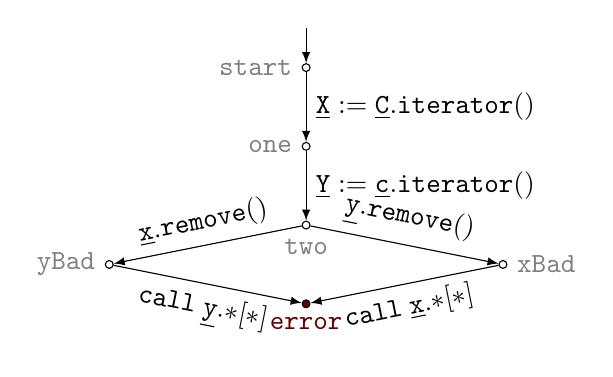
\begin{tikzpicture}
  \def\x{2.5}
  \tikzset{vertex/.style={draw,circle,inner sep=1pt}}
  \tikzset{transition/.style={->,>=latex}}
  \tikzset{every label/.style={gray}}
  \node[vertex] (start) at (0,0) [label=left:\texttt{start}] {};
  \node[vertex] (gotOne) at (0,-1) [label=left:\texttt{one}] {};
  \node[vertex] (gotTwo) at (0,-2) [label=below:\texttt{two}] {};
  \node[vertex] (xBad) at (1*\x,-2.5) [label=right:\texttt{xBad}] {};
  \node[vertex] (yBad) at (-1*\x,-2.5) [label=left:\texttt{yBad}] {};
  \node[vertex,fill=darkred] (error) at (0,-3) [label=below:\textcolor{darkred}{\texttt{error}}] {};
  \draw[transition] (0,0.5)--(start);
  \draw[transition] (start)--node[right]{$\pattern X:=\pattern C.\mathtt{iterator}()$} (gotOne);
  \draw[transition] (gotOne)--node[right]{$\pattern Y:=\pattern c.\mathtt{iterator}()$} (gotTwo);
  \draw[transition] (gotTwo) -- node[sloped,above]{$\pattern y.\mathtt{remove}()$} (xBad);
  \draw[transition] (gotTwo)--node[sloped,above]{$\pattern x.\mathtt{remove}()$} (yBad);
  \draw[transition] (xBad)--node[sloped,below]{$\mathtt{call}\;\pattern x.{*}[*]$} (error);
  \draw[transition] (yBad)--node[sloped,below]{$\mathtt{call}\;\pattern y.{*}[*]$} (error);
\end{tikzpicture}
\caption{A first example: Diagram of safety property}
\label{fig:first.diagram}
\end{figure}
\begin{figure}
\begin{Verbatim}[commandchars=\\\{\}]
property InvalidateOtherIterators
  using prefix java.util.Collection
  using prefix java.util.Iterator
  start -> one:  \pattern{X} := \pattern{C}.iterator()
  one -> two:    \pattern{Y} := \pattern{c}.iterator()
  two -> yBad:   \pattern{x}.remove()
  two -> xBad:   \pattern{y}.remove()
  jBad -> error: call \pattern{y}.*[*]
  iBad -> error: call \pattern{x}.*[*]
\end{Verbatim}
\caption{A first example: Safety property}
\label{fig:first.topl}
\end{figure}
\begin{figure}
{\def\s#1{\text{\Verb@#1@}}
 \def\m#1{\PY{n+na}{#1}}
 \def\t#1{\mathtt{#1}}
\begin{align*}
&\{(\start,[])\} \\
&\s{Iterator<Integer> i = c.\m{iterator}();} \\
&\text{assume {\tt c} holds $1$, and {\tt i} holds $2$ } \\
&\{(\start,[]), (\t{one},[c:1,x:2])\} \\
&\s{Iterator<Integer> j = c.\m{iterator}();} \\
&\text{assume {\tt j} holds $3$} \\
&\{(\start,[]), (\t{one},[c:1,x:3]),(\t{two},[c:1,x:2,y:3])\} \\
&\s{i.\m{next}();} \\
&\{(\start,[]), (\t{one},[c:1,x:3]),(\t{two},[c:1,x:2,y:3])\} \\
&\s{i.\m{remove}();} \\
&\{(\start,[]), (\t{one},[c:1,x:3]),(\t{yBad},[c:1,x:2,y:3])\} \\
&\s{j.\m{next}()} \\
&\{(\start,[]), (\t{one},[c:1,x:3]), (\error,[c:1,x:2,y:3])\}
\end{align*}}
\caption{A first example: Running step by step}
\label{fig:first.steps}
\end{figure} % >>>

\autoref{fig:first.steps} shows an execution of the program and of an automaton for the property \texttt{InvalidateOtherIterators}.
The lines \{in curly brackets\} describe the state of the automaton;
the lines in \texttt{monotype} show the statements that execute;
the other lines are comments.
At a given moment, the automaton has a set of active states.
A state is a pair of a vertex and a store.
The store is a memory that holds (automaton) variables.
Technically, it is a finite partial map from variables to values.
(A partial finite map is sometimes called a \emph{dictionary}.)

\begin{notation}
We write $[k_1:v_1,k_2:v_2]$ for the finite partial map that maps key~$k_1$ to value~$v_1$, and key~$k_2$ to value~$v_2$.
The empty map is denoted by~$[]$.
\end{notation}

The automaton has variables $x$,~$y$, and~$c$.
At vertex \texttt{one} the variables $x$~and~$c$ are initialized;
at vertex \texttt{two} the variables $y$,~$y$ and~$c$ are initialized.
Being at vertex \texttt{one} means that $x$~is an iterator for~$c$;
being at vertex \texttt{two} means that $x$~and~$y$ are two iterators for the same collection~$c$.
There is a program variable~\Verb@c@ and an automaton variable~$c$.
The same name was chosen because the two variables always hold the same value in this example.
In general, however, program variables and automaton variables live in different name-spaces.

\begin{notation}
Program variables are typeset in \Verb@monotype@ (\Verb@c@,~\Verb@i@,~\Verb@j@).
Automaton variables are typeset in \textit{italics} ($c$,~$x$,~$y$).
Program variables appear in the program;
automaton variables do \emph{not} appear in the property.
Instead, automaton variable \emph{patterns} appear in the property, and they are typeset in \texttt{\underline{underlined monotype}} (\pattern c,~\pattern C, \pattern x, \pattern X, \pattern y,~\pattern Y).
\end{notation}

As it will become apparent below, the interaction between patterns and automata memory is as follows: uppercase patterns write to the automaton memory, and lowercase patterns read from the automaton memory and act as a guard on the transition.

\paragraph{Step~1.}

Initially, only the state $(\start,[])$ is active.
The outgoing transition of vertex \start is labeled by \[\pattern X:=\pattern{C}.\mathtt{iterator}()\] and the first executed statement is \verbline[.]{i = c.\PY{n+na}{iterator}()}
A method call matches a label when
\begin{itemize}
\item[(a)] the called method matches the method pattern, and
\item[(b)] the program values match their corresponding patterns.
\end{itemize}
By definition, any value matches an Uppercase pattern.
Here, the values of \Verb@i@~and~\Verb@c@ trivially match the patterns \pattern X~and~\pattern C.
The method itself also matches the method pattern, but for a slightly more complicated reason than it appears.
For simplicity, we ignore argument types and identify Java methods only by their fully qualified name and by their arity.
The called method \texttt{iterator} is in the class \texttt{ArrayList} and has arity~$1$.
We identify it as follows.
\verbline{java.lang.ArrayList.iterator[1]}
Without \texttt{using prefix} directives, the method pattern would be \Verb@iterator[1]@.
With the directives, however, the pattern is the following.
\begin{align*}
&\text{\Verb@java.util.Collection.iterator[1]@} \\
&\text{\Verb@java.util.Iterator.iterator[1]@}
\end{align*}
It means that these two methods \emph{and} all those that override them match.
Here, \texttt{ArrayList} implements \texttt{Collection}.

All conditions are met to perform the transition from \start to \texttt{one}.
When the transition is performed the values that matched \pattern X~and~\pattern C are written in the automaton variables $x$~and~$c$.
For concreteness, let us assume these values are $1$~and~$2$.
After the transition is performed, the state $(\mathtt{one},[c:1,x:2])$ is active.

\paragraph{Step~2.}
For the second step the statement to be executed is \verbline[.]{j = c.\PY{n+na}{iterator}()}
Now we need to consider the two active states in turn\footnote{The state $(\start,[])$ is a special state that is always active.
Conceptually, the vertex \texttt{start} has a self-loop on it that always matches.}:
\[\{(\start,[]), (\texttt{one},[c:1,x:2])\}\] 
For $(\start,[])$ exactly the same reasoning as step 1 holds and the result is that \[(\texttt{one},[c:1,x:3])\] is active after the second step.
Note that now the automaton variable~$x$ remembers the value of the program variable~{\tt j}.
For \[\texttt{(one},[c:1,x:2])\] we look at the transition outgoing from vertex {\tt one} which has the label \[\pattern{Y}:=\pattern{c}.\mathtt{iterator}();\]
The method and the uppercase pattern~$\pattern Y$ match in the same way as before.
The lowercase pattern $\pattern c$ matches only the value that is held by the automaton variable~$c$.
In this case, the transition $\texttt{one}\to\texttt{two}$ is performed because the program variable~{\tt c} still refers to the same collection it did when the transition $\start\to\texttt{one}$ was performed.

\paragraph{Step~3.}

The third step involves the statement
\[\text{\Verb+\PY{n}{i}\PY{o}{.}\PY{n+na}{next}\PY{o}{(}\PY{o}{)}\PY{o}{;}+}\]
which matches no label of outgoing transitions of the currently active states (i.e., $\start$, {\tt one}, and {\tt  two}).
Therefore, although the program proceeds, the set of active states in the automaton remain unchanged.

\paragraph{Step~4.}

In the fourth step, the transition $\texttt{two}\to\texttt{yBad}$ is performed.
Notice that the pattern $\pattern{x}.\mathtt{remove}()$ does not have a left-hand side, which simply means that the returned value is irrelevant for this transition.
The states corresponding to vertices $\start$ and {\tt one} remain unchanged, because their outgoing transitions do not match.
However,  the outgoing transition of state {\tt two} can fire, and therefore {\tt yBad} becomes active.

\paragraph{Step~5.}

For the fifth and final step, the statement to be executed is \verbline[.]{j.\PY{n+na}{next}()}
The label of the outgoing transition  \[\mathtt{call}\;\pattern{y}.{*}[*]\] of the active state $(\texttt{yBad},[c:1,x:2,y:3]),$
has two distinguishing features: the~$*$ as a method name and the tag \texttt{call}.
As before, in order to match the method name, the following prefixes are prepended  
\begin{align*}
&\text{\Verb@java.util.Collection.*[*]@} \\
&\text{\Verb@java.util.Iterator.*[*]@}
\end{align*}
Then the $*$s are expanded, taking into account the \texttt{CLASSPATH}.
We have a match because the expansion \verbline{java.util.Iterator.next} is overridden by the method that is actually called.

The tag {\tt call} is used when we want the automaton to take a transition precisely at call-time of a method invocation.
This is useful when we need to distinguish different events that may happen during a method invocation with different automata states (e.g., at call-time or return-time or in between).
In our example, the automaton expresses that the simple fact that a {\tt j}'s method is called from a {\tt yBad} state is enough for activating an error state. Notice that this is different from a tag of the type $\pattern X:=\pattern C.\mathtt{iterator}()$ which expects the transition to involve all the events of the method invocation, from call-time till the return-time.

\medskip
The execution we stepped through violates the property \textit{InvalidateOtherIterators} because the vertex \texttt{error} is reached.
Notice that in order to find a counterexample we need to keep track of the relation between several objects, in particular that iterators {\tt i} and {\tt j} are for the same collection {\tt c}.
In practice, programmers tend to violate this property when the code is more involved and uses the shorthand notation for iteration $\mathbf{for}(T\;x:c)$.

% >>>
\subsection{More Iterators} \label{sec:examples.iterators} % <<<

Other interesting properties of iterators~\cite{dblp:conf/oopsla/naeeml08,dblp:conf/sigsoft/boddenlh08,haack2009} are also easy to express in TOPL\null.

\medskip\emph{Modifying a collection invalidates all its existent iterators:}
\delimitVerbatim
\begin{Verbatim}
property ModificationInvalidatesIterators
  using prefix java.util.{Collection,Iterator}
  start -> iterating:     I := C.iterator()
  iterating -> modified:  c.add(*), c.remove(*)
  modified -> error:      call i.*[*]
\end{Verbatim}
\delimitVerbatim
This property should list all the methods of \textit{Collection} that mutate it.
If classes that implement \textit{Collection} add mutating methods, then those should be included as well.
This ``abstraction leak'' is intrinsic to Java where sub-classing is not sub-typing.

\medskip\emph{Iterators should advance only if they are not exhausted:}
\delimitVerbatim
\begin{Verbatim}
property UnsafeIteratorNext
  using prefix java.util.{Collection,Iterator}
  start -> iterating:         I := *.iterator()
  iterating -> notExhausted:  true := i.hasNext()
  notExhausted -> iterating:  i.next()
  iterating -> error:         i.next()
\end{Verbatim}
\delimitVerbatim
The transition from \Verb@iterating@ to \Verb@notExhausted@ matches when \Verb@hasNext@ returns \Verb@true@.
In general, Java literals act as guards on transitions.

\medskip\emph{Method \Verb@remove@ may only be called after \Verb@next@:}
\delimitVerbatim
\begin{Verbatim}
property RemoveBeforeNext
  using prefix java.util.{Collection,Iterator}
  start -> created: I := *.iterator()
  created -> ok:    i.next()
  created -> error: i.remove()
\end{Verbatim}
\delimitVerbatim
TOPL is designed to track properties involving multiple objects.
However, properties involving a single object are also easy to express.
The vertex \Verb@ok@ is not special.
The purpose of the transition going to \Verb@ok@ is to deactivate the state with vertex \Verb@created@.

\medskip
We have now seen four properties of iterators.
Each corresponds to a simple English sentence.
It is possible to use only one TOPL property.
However, there is no advantage of doing so.

% >>>
\subsection{Resources} % <<<

Many resources impose two temporal properties:
Before being used they must be acquired;
after being acquired they must be eventually released.
Resources include memory, files, sockets, locks.
Memory must be allocated before reading or writing and should eventually be deallocated;
files must be opened before reading or writing and should eventually be closed;
sockets must be created before sending and receiving data and should eventually be closed;
locks should be acquired before accessing the memory they protect and should eventually be released.
Resources are usually represented by objects.
\delimitVerbatim
\begin{Verbatim}[commandchars=\\\{\}]
\PY{k+kd}{interface} \PY{n+nc}{Resource} \PY{o}{\PYZob{}}
  \PY{k+kt}{void} \PY{n+nf}{acquire}\PY{o}{(}\PY{o}{)}\PY{o}{;}
  \PY{k+kt}{void} \PY{n+nf}{use}\PY{o}{(}\PY{o}{)}\PY{o}{;}
  \PY{k+kt}{void} \PY{n+nf}{release}\PY{o}{(}\PY{o}{)}\PY{o}{;}
\PY{o}{\PYZcb{}}
\end{Verbatim}

\delimitVerbatim
To create a resource, we use the static method \Verb@makeResource@.

\medskip\emph{A resource must be acquired when used:}
\delimitVerbatim
\begin{Verbatim}
property ResourceSafety
  start -> released:    R := makeResource()
  released -> error:    r.use()
  released -> acquired: r.acquire()
  acquired -> released: r.release()
\end{Verbatim}
\delimitVerbatim
In simple cases, resources cannot repeatedly move between the states \Verb@released@ and \Verb@acquired@.
\delimitVerbatim
\begin{Verbatim}
property ResourceSafetySimple
  start -> acquired:    R := makeResource()
  acquired -> released: r.release()
  released -> error:    r.use()
\end{Verbatim}
\delimitVerbatim
The following examples in this subsection only cover the case when \Verb@acquire@ must be called explicitly.

\medskip\emph{A resource must not be released twice:}
\delimitVerbatim
\begin{Verbatim}
property DoubleRelease
  start -> released:    R := makeResource()
  released -> acquired: r.acquire()
  acquired -> released: r.release()
  released -> error:    r.release()
\end{Verbatim}
\delimitVerbatim
Similarly, one can express that a resource must not be acquired twice.

\medskip\emph{A resource must eventually be released:}
\delimitVerbatim
\begin{Verbatim}
property ResourceLeak
  start -> released:    R := makeResource()
  released -> acquired: r.acquire()
  acquired -> released: r.release()
  acquired -> error:    return Main.main[1]
\end{Verbatim}
\delimitVerbatim
TOPL is designed for safety properties, which have finite counter-examples.
It is not possible to express the lack of resource leaks in non-terminating programs.
It is possible, however, to check if resources are leaked when the program terminates.

% >>>
\subsection{\textsc{Slic} Queue} % <<<

\textsc{Slic}~\cite{ball2002} is the property language of SLAM~\cite{dblp:conf/cav/ballr01}.
Its authors give the following interesting example.

\medskip\emph{A queue may contain at most three zeros:}
\delimitVerbatim
\begin{Verbatim}
property TooManyZeros
  start -> cnt0: Q := makeQueue()
  cnt0 -> cnt1:  q.put(0)
  cnt1 -> cnt2:  q.put(0)
  cnt2 -> cnt3:  q.put(0)
  cnt3 -> error: q.put(0)
  cnt3 -> cnt2:  0 := q.get()
  cnt2 -> cnt1:  0 := q.get()
  cnt1 -> cnt0:  0 := q.get()
\end{Verbatim}
\delimitVerbatim
The vertex \texttt{cnt}\textit{x} means that there are $x$~zeros in~$q$.
A natural generalization is to allow at most $n$~zeros.
The size of the TOPL property text grows linearly with~$n$.
A better solution would be to allow incrementing and decrementing of automaton variables when transitions are performed.
However, it is unclear if such properties arise in practice, so we chose to keep TOPL simple.
Moreover, we will see later (\autoref{sec:syntax.topl}) that TOPL is translated to an intermediate language that does support such actions.

% >>>
\subsection{Sorter and Comparator}\label{sec:examples.sorter} % <<<

This section is inspired by the higher-order temporal properties of Disney et al.~\cite{disney2011}.
We adapt their first motivating example to the object-oriented setting.
Consider the following interface fragments.
\delimitVerbatim
\begin{Verbatim}[commandchars=\\\{\}]
\PY{k+kd}{interface} \PY{n+nc}{Comparator}\PY{o}{<}\PY{n}{T}\PY{o}{>} \PY{o}{\PYZob{}}\PY{o}{\PYZcb{}}
\PY{k+kd}{interface} \PY{n+nc}{Sorter}\PY{o}{<}\PY{n}{T}\PY{o}{>} \PY{o}{\PYZob{}}
  \PY{k+kt}{void} \PY{n+nf}{sort}\PY{o}{(}\PY{n}{Comparator}\PY{o}{<}\PY{n}{T}\PY{o}{>} \PY{n}{c}\PY{o}{)}\PY{o}{;}
\PY{o}{\PYZcb{}}
\end{Verbatim}

\delimitVerbatim
Sorter objects implement comparison-based sorting algorithms.

\medskip\emph{The \Verb@sort@ method is not recursive:}
\delimitVerbatim
\begin{Verbatim}
property RecursiveSort
  using prefix Sorter
  start -> inSort: call sort[*]
  inSort -> ok:    return sort[*]
  inSort -> error: call sort[*]
\end{Verbatim}

\medskip\emph{A comparator may only be used by its sorter:}
\delimitVerbatim
\begin{Verbatim}
property ReusedComparator
  using prefix Sorter
  start -> x: call S.sort(C)
  x -> error: <!s> call c.*[*]
\end{Verbatim}
\delimitVerbatim
The state $(x,[c:-;s:-])$ is active when comparator~$c$ was given to sorter~$s$.
The pattern within \Verb@<@angle brackets\Verb@>@ is matched against the value of \textbf{this}.
The pattern \Verb@!s@ matches when the pattern \Verb@s@ does not match.

% >>>
\subsection{Atomicity} % <<<

Another interesting property discussed by Disney et al.~\cite{disney2011} in the context of functional languages is atomicity.

\medskip\emph{Method~\Verb@m@ should be atomic:}
\delimitVerbatim
\begin{Verbatim}
property NotAtomicM
  start -> inM: call m[*]
  inM -> ok:    return m[*]
  inM -> error: call badCall[*]
\end{Verbatim}
\delimitVerbatim
All the events that should not intervene between the call to~\Verb@m@ and the return from~\Verb@m@ must be explicitly mentioned.
Otherwise, if the granularity for atomicity is implicit, then it is easy for users to make mistakes.

% >>>
\subsection{JDBC} \label{sec:examples.jdbc} % <<<

\rg{TODO}
\par\medskip\noindent
\begin{Verbatim}
property BlaBla
\end{Verbatim}

% >>>
% >>>
\section{Syntax}\label{sec:syntax} % <<<

We begin the systematic presentation of TOPL with its syntax (\autoref{sec:syntax.topl}).
Before moving on to semantics (\autoref{sec:semantics}) we shall also introduce the syntax of SOOL, a \textbf simple \textbf object-\textbf oriented programming \textbf language (\autoref{sec:syntax.sool}).
Our prototype implementation is an interpreter for SOOL programs that dynamically checks TOPL properties.

\subsection{TOPL and iTOPL}\label{sec:syntax.topl} % <<<

% plan
% - two languages
% - language for users
% - language for semantics
% - desugaring translation

TOPL aims to be intuitive:
Labels look like method calls, there is a shorthand notation for parallel transitions, there is an implied loop on the vertex \start, the \texttt{using prefix} directive offers some extra convenience, and so on.
From the point of view of semantics, however, these conveniences are in the way.
For this reason we also define iTOPL (\textbf inner TOPL), an even simpler language into which TOPL is desugared.

\autoref{fig:syntax.topl} shows the syntax of TOPL\null.
A property has a name, a set of \texttt{using} directives, and a set of transitions.
Each transition has an arc (directed edge) and labels.
Each arc has a source vertex and a target vertex.
All vertices are identified by their name.
Labels look roughly like method calls.
Each label has a method pattern that is used to identify the set of methods to which the label refers.
In the simple case, a method pattern consists of a string pattern for the name of the method and an integer that specifies the method arity.
(For simplicity, TOPL does not use the static types of arguments to distinguish between overloaded methods.)
The more interesting case is when there are value patterns for each argument and perhaps even for the context and the result.
The context pattern appears \Verb@<@surrounded by angle brackets\Verb@>@ at the beginning of the label and is matched against the value of the special variable \textbf{this}.
Transitions should typically be tagged with \texttt{call} or \texttt{return} to specify exactly at what time they should be performed (see \autoref{sec:semantics.itopl} for details).

\begin{figure}
\grammar{
  Property& \b{property} Identifier Using\* Transition\* \cr
  Using& \b{using prefix} StringPattern \cr
  Transition& Arc \b: Label \(\b, Label\)\* \cr
  StringPattern& \(Letter \| \b. \| \b*\)\+ \cr
  Arc& Vertex \b{->} Vertex \cr
  Label& Context\? Tag\? MethodPattern \cr
  Vertex& Identifier \cr
  Context& \b< ValuePattern \b> \cr
  Tag& \b{call} \| \b{return} \cr
  MethodPattern& ResultPattern\? NamePattern ArgumentsPattern \cr
  ResultPattern& ValuePattern \b{:=} \cr
  NamePattern& StringPattern \cr
  ArgumentsPattern& \b( \(ValuePattern \(\b, ValuePattern\)\*\)\? \b) \cr
  ArgumentsPattern& \b[ IntegerPattern \b] \cr
  ValuePattern& \b* \| Literal \| UppercaseId \| \b!\? LowercaseId \cr
  IntegerPattern& \b* \| IntegerLiteral \cr
}
\caption{Syntax of TOPL}
\label{fig:syntax.topl}
\end{figure}

\begin{notation}
\rg{TODO: Grammar: italics, monotype, superscript, and so on.}
\end{notation}

There are three types of patterns used in TOPL---for strings, for integers, and for values.
String patterns match method names and may use wildcards.
(For simplicity, TOPL does not use full regular expressions as string patterns.)
\rg{I also used \Verb@{a,b}@ so I need to say something like `POSIX path patterns.'}
Integer patterns specify method arities.
Value patterns are the most interesting.
\rg{TODO: Explain wildcard and literals for value patterns.}
For each automaton variable \Verb@var@ there are three associated patterns.
The uppercase pattern \Verb@Var@ matches any value and writes it in the automaton variable \Verb@var@.
The lowercase pattern \Verb@var@ reads the value of the automaton variable \Verb@var@ and only matches that value.
The negated lowercase pattern \Verb@!var@ reads the value of the automaton variable \Verb@var@ and only matches different values.

A TOPL property is \emph{well-formed} when it satisfies the following conditions.
\begin{itemize}
\item Labels must contain uppercase value patterns at most once.
\item Any use of a lowercase patterns must be guaranteed preceded by a
  use of the corresponding uppercase pattern.
  In other words, automaton variables must be written before being read.
\end{itemize}
\dinocomment{how do we guarantee that properties are well formed? Maybe we should say that we assume in the following that they are.}
\autoref{fig:syntax.itopl} shows the syntax of iTOPL\null.
The missing productions (eg. $Arc$) are the same as for TOPL\null.
Each transition now has exactly one label.
Each label is a list of (guard, action) pairs.
Each guard is some boolean combination of atomic guards.
Each action is a sequence of atomic actions.
Both guards and actions refer to some implicit array of values using an index (see \autoref{sec:semantics.itopl}).
Atomic guards compare values either with automaton variables (\textit{Identifier}) or with constants (\textit{Literal}).
Atomic actions write values into automaton variables.
There is also an atomic guard that matches against method calls and always specifies a tag \Verb@call@ or \Verb@return@, but never involves examining any values.

\begin{figure}
\grammar{
  Property& \b{property} Identifier Transition\* \cr
  Transition& Arc \b: Label \cr
  Label& \(\b(Guard Action\b)\)\* \cr
  Guard& AtomicGuard \| Guard \(\(\b{\&}\|\b|\) Guard\)\* \cr
  Action& \(AtomicAction \(\b, AtomicAction\)\*\)\? \cr
  AtomicGuard& \b! Guard \cr
  AtomicGuard& \b[ ValueIndex \b] \b= \(Identifier \| Literal\)\cr
  AtomicGuard& \(\b{call} \| \b{return}\) NamePattern \b[ IntegerPattern \b] \cr
  AtomicGuard& \b{true} \cr
  AtomicAction& Identifier \b{:=} \b[ ValueIndex \b] \cr
  ValueIndex& IntegerLiteral \cr
}
\dinocomment{why many syntactic categories are called AtomicGuard?}
\rlp{Is it the case that $Action ::= (AtomicAction)^*$ or not?}
\rg{It depends on whether we give an abstract syntax or a concrete syntax.
I prefer a concrete syntax.}
\rlp{Why is $!Guard$ an $AtomicGuard$?}
\rg{See \Verb@ReusedComparator@ in \autoref{sec:examples.sorter}.
I think there were some other examples where we needed it, but I can't remember now.}
\rlp{Is it the case that $\set{Value} = (Identifier | Literal)$?}
\rg{\set{Value} is a set; \textit{Identifier} and \textit{Literal} are syntactic categories that can be used in Java to denote values.}
\caption{Syntax of iTOPL}
\label{fig:syntax.itopl}
\end{figure}

\rg{TODO: Present desugarings---things like methods names, going from patterns to guards and actions.}

% >>>
\subsection{Translating TOPL into iTOPL}\label{sec:syntax.desugaring} % <<<
The main translation is that of TOPL labels into iTOPL labels. To
illustrate how that works, let $\mathit{Context}\ \mathit{Tag}\
\mathit{MethodPattern}$ be a TOPL label. If $$
% >>>
\subsection{SOOL}\label{sec:syntax.sool} % <<<

SOOL is a subset of existing object-oriented languages.
It has classes, assignments, and method calls.
It should be possible to use TOPL with any language that is a superset of SOOL\null.

\autoref{fig:syntax.sool} shows a big part of SOOL's syntax.
Expressions, which do not have side-effects, are missing.

\begin{figure}
\grammar{
  Program& Class\* Main\cr
  Class& \b{class} Identifier Member\* \cr
  Main& \b{main} Body \cr
  Member& Type Identifier & data \cr
  Member& Type Identifier \b( Formals\? \b) Body & code\cr
  Body& Statement\* \cr
  Formals& Type Identifier \(\b, Type Identifier\)\* \cr
  Statement& \b{return} Expression & return\cr
  Statement& Reference \b{:=} \b{new} & allocate \cr
  Statement& Reference \b{:=} \b* & read \cr
  Statement& Reference \b{:=} Reference \b( Actuals\? \b) & call \cr
  Statement& \b{do} Body \b{while} Expression Body &loop\cr
  Statement& \b{if} Expression Body \b{else} Body &test\cr
  Reference& Expression \b. Identifier \cr
  Actuals& Expression \(\b, Expression\)\* \cr
}
\rlp{Is $Body$ normally called $Block$?}
\rg{\emph{I} normally call it \textit{Body}.
I think the C standard calls it ``composed statement.''
(Conditionals and loops are ``control-flow statements,'' I think.)
In summary:
I don't know what's more common, so feel free to change.}
\caption{(Partial) Syntax of SOOL}
\label{fig:syntax.sool}
\end{figure}

% >>>
% >>>
\section{Semantics}\label{sec:semantics} % <<<

A program's semantics is a set of event traces;
an automaton's semantics is also a set of event traces.
We say that a program \emph{violates} a property when their sets of traces intersect.
In other words, properties encode bad executions, rather than good executions.

\begin{notation}
\rg{TODO: Sets, $\to$, $\times$, $(a,b)$, and so on.}
\end{notation}

\subsection{Semantics of iTOPL}\label{sec:semantics.itopl} % <<<
\textcolor{lightblue}{[Start of rewrite]}\\
Each property gives rise to an automaton defined over the labeled multigraph $(V, E)$ given
by the transitions: $V$ is the set of vertices mentioned as endpoints of
the arcs and $E$ is the set of labeled edges mentioned by the
transitions.
\rg{Let's use `arc' consistently for `directed edge.'}

For the property to be well-formed there must be a vertex start and a
vertex error.
%\rlp{Is this correct, and should it be part of the grammar?}
%\rg{I think it should not be part of the grammar.
%At the moment it is not enforced by the static checker, but it should.
%So I'd say that what you say is correct.}
\rlp{Somewhere note distinction between start vertex and start
  state.}

The automaton takes as input a list of events carrying values.
\rg{This is ambiguous to parse: ``(list of events) carrying values'' or ``list of (events carrying values)''?}
For values, we assume a countable set \set{Value} and for events we assume
a finite set \set{Event} of events with known arity.
\rg{Does the cardinality of \set{Value} matter?}
\rg{Does the cardinality of \set{Event} matter?}
\rg{I think it should be made clear that events \emph{contain} values.
It's conceivable to interpret this paragraph as saying that the input has type $(\mathit{event}*\mathit{value}\,\mathit{list})\,\mathit{list}$.}

We will now describe how the automaton reacts to events, specifically
how labels are evaluated. As this is a slightly non-standard
automaton, there are some important things to point out. Firstly, the
state of the automaton is not just a vertex but also a store. 
That is, there is an array of automaton variables, referred to by
index in the guards and actions, and the state of the automaton is
given by specifying the vertex in the graph as well as the value of
all automaton variables.

We model stores as partial functions with finite domain (sometimes called dictionaries):
\rg{Do you skip equation numbers on purpose?}
\[
\set{Store} = \N \pmap \set{Value}
\]
\rg{Why did you replace \set{Variable} by $\N$?
I got \set{Variable} from separation logic articles.
I know the Java code from the plane uses $\N$, but I'd say that's an implementation choice.}
And so a state of the automaton has the type
\[
\set{State} = \set{Vertex}\times\set{Store}
\]
Given the state of the automaton and an event we would like to know
which transitions are available. But actually, we do not have enough
information to determine that. This is a consequence of the second
slightly non-standard aspect of our automatons, namely that each label
carries not only a single guard but potentially a list of guards.
We call the length of this list, the \emph{depth} of the transition.
\rg{I said `length' in \autoref{sec:dynamic}, which needs rewriting anyway.
Should we say `transition depth' everywhere from now on?}
\rlp{Yes, let us do that.}

In order for a transition to be available, all the guards along its
list have to evaluate to true. We will describe this evaluation in a
moment, but now we note that each guard along the transition consumes
an event. Thus we have to know a whole prefix of the trace of events
inorder to see if a transition is enabled, as long as the depth of the
transition.

A further consequence is, that the following events to be received are
not the same at the end of each enabled transition. If two transitions
turn out to be enabled, one with depth 2 and the other with depth 5,
then the end state of the first transition will see the third event of
the trace next, while the end state of the second transition will see
the sixth event next. For this reason, it is necessary to keep track
of which events are next to be received by each state during a run of
the automaton.

To formalize this book keeping, we introduce the notion of
\emph{execution state}. Execution states have the type
\[
\set{ExeState} = \set{State}\times\set{Trace}
\]
where the first component records the state of the automaton (vertex
and store) and the second component records the remaining trace of
events for that state.

We now describe when transitions are enabled. For this we have to look
at labels. A label is a list of pairs of guards and actions. A
guard compare the values in an event with those in a store and
concludes either pass or no pass:
\[
\set{Guard} = \set{Event}\to\set{Store}\to2
\]
if the event passes, the corresponding action is taken on that event.
Actions modify the store, using values from an event:
\[
\set{Action} = \set{Event}\to\set{Store}\to\set{Store}
\]
In order for a transition of depth $n$ to be enabled for a trace of
events, the first $n$ events of the trace has to pass the $n$ guards
on the label with the stores modified by the guards:
\rg{If guards take a pair then you should also change \set{Guard} above.
Same for \set{Action}.}
\[
\begin{array}{c l}
& \mathit{enabled}((g_1, a_1), \ldots, (g_n, a_n); e_1, \ldots, e_n; s) \\
 = &
g_1(e_1, s_0)\ \land\ \ldots\ \land\ g_n(e_n, s_{n-1}) 
\end{array}
\]
where
\begin{align}
  s_0 &=  s \\
  s_i &= a_i(e_i, s_{i-1}) &&\text{for $i\in1.\,.\,n$}
\end{align}
If the transition is enabled and taken, the store for the vertex at the end of the arc will be $s_n$.
\rg{I was saying `matched' and `performed'.
I like `enabled' better than `matched', because the latter seems more overloaded.
I'm not sure about `taken'.
I chose `performed' over taken because it suggests there are actions being done.}
\rlp{I like `taken' because in english a transition can be taken,
  meaning chosen, and an action can be taken, meaning
  performed. `Performing' a transition sounds a bit wrong.}

And now we reach the final slightly non-standard aspect of our
automatons, namely that if no transitions are enabled for a given
state and trace of events, the automaton does not get stuck but is
allowed to consume one event without changing its state. Note that
this is not equivalent to an implied self-loop on all states, as
dropping events is not allowed if there are any enabled
transitions. In that case one of the enabled transitions is taken and
the automaton execution state becomes $((v, s_n), \mathit{events}_n)$, where $v$ is the vertex at the
end of the arc of the transition, $s_n$ is defined as above and
$\mathit{events}_n$ is the current executions state's event trace with the first
$n$ events dropped.
\rg{An example would help to understand this paragraph.}

We can define a predicate that determine the possible execution state transitions
\[
\mathit{Step}\in\set{ExeState}\to\set{ExeState}\to2
\]
this predicate is defined in \autoref{fig:adStep}.
From this we can define a non-deterministic step function, where all
enabled transitions are taken:
\begin{align}
\mathit{NdetStep}&\in(\set{ExeState}\to2)\to\set{ExeState}\to2\\
%\mathit{NdetStep}\;S&=(\bigcup \mathit{Step})\;S \label{eq:ndetstep}
\mathit{NdetStep}\;S&=\{ s \mid \exists s'\in S.\ \mathit{Step}(s', s) \} \label{eq:ndetstep}
\end{align}
An iterated version of \textit{NdetStep} is useful for defining reachable states.
We define it as the least fixed point for the following equation.
\begin{align}
\mathit{NdetStep}^\star\;S &= S \cup \mathit{NdetStep}^\star\;(\mathit{NdetStep}\;S)
\end{align}
\rlp{Should this really include 0-sized steps?}
\rg{I prefer to keep epsilon transition, unless there is a good reason to special-case them.}
Finally, we can define the set of traces described by an automaton:
\[
\{ e \mid
\exists\sigma'e',\;((\mathtt{error},\sigma'),e')\in\mathit{NdetStep}^\star\;\{((\mathtt{start},[]),e)\}
\}
\]
These are the traces that drive the automaton from the \texttt{start} vertex (with an empty store) to the \texttt{error} vertex.
\ \\ \textcolor{lightblue}{[End of rewrite]}\\


In the following, let $n=\{0,1,\ldots,n-1\}$ and let \set{Value} denote a generic set of values.
Each event has a tag and carries an array of values.
\begin{align}
\set{Event}&=\bigcup_{n\in\N}\set{Tag}_n\times(n\to\set{Value})
\end{align}
We assume that these basic sets are disjoint.
Traces are finite.
\begin{align}
\set{Trace}=\bigcup_{n\in\N} n\to\set{Event} \label{eq:trace}
\end{align}
Intuitively, the program outputs a trace that drives the automaton.
\dinocomment{Only one? I would say a set of traces. Right?}
\dinocomment{Can we give the reader an intuitive reason why the event are of that form? Also, why is Tag indexed with $n$?}
The automaton is defined on top of a finite multi-graph.
The automaton is an array of transitions.
Each transition has an edge and an array of labels.
Each edge has a source vertex and a target vertex.
Each label is a (guard, action) pair.
There are at least two vertices.
\begin{align}
\set{Automaton} &= \bigcup_{n\in\N} n \to \set{Transition} \\
\set{Transition} &= \set{Edge}\times \bigcup_{n\in\N} n\to\set{Label} \\
\set{Edge}&=\set{Vertex}\times\set{Vertex} \\
\set{Label}&=\set{Guard}\times\set{Action} \\
\{\mathtt{start},\mathtt{error}\}&\subseteq\set{Vertex}
\end{align}
The deterministic state contains a store of values.
\dinocomment{this deterministic state seems to come out of the blue.
\rg{What do you mean?
This is its definition.}}
\dinocomment{I think it would be good to give an introduction about the determinist state. What is it? Why it is needed?
etc. Just the definition at this point leave the reader wondering...}
A store is a finite partial map from automaton variables to values.
We also define an automaton deterministic execution state, which includes the input to be processed.
\begin{align}
\set{Store}&=\set{Variable}\pmap\set{Value} \\
\set{AState}&=\set{Vertex}\times\set{Store} \label{eq:astate} \\
\set{EAState}&=\set{AState}\times\set{Trace} \label{eq:eastate}
\end{align}
Guards compare the values in an event with those in a store.
Actions modify the store, using values from an event.
\begin{align}
\set{Guard}&=\set{Event}\to\set{Store}\to2 \\
\set{Action}&=\set{Event}\to\set{Store}\to\set{Store}
\end{align}
The automaton deterministic step function evolves the execution state.
\begin{align}
\mathit{adStep}\in\set{EAState}\to\set{EAState}\to2 \label{eq:adstep}
\end{align}
\begin{example}
Consider an automaton in state~$s_1$.
The input is a trace~$e_1e_2$ obtained by concatenating traces $e_1$~and~$e_2$.
The automaton must make a nondeterministic choice out of some alternatives.
A feasible alternative might be to consume $e_1$ and move to state~$s_2$.
For this, we write $(s_2,e_2)\in\mathit{adStep}(s_1,e_1e_2)$.
(We write $x\in f$ to mean that $f(x)=1$.)
\end{example}
The nondeterministic step is defined in terms of~\textit{adStep}.
\begin{align}
\mathit{anStep}&\in(\set{EAState}\to2)\to\set{EAState}\to2\\
\mathit{anStep}\;S&=\bigcup \mathit{map}\;\mathit{adStep}\;S \label{eq:anstep}
\end{align}
An iterated version of \textit{anStep} is useful for defining reachable states.
We define it as the least fixed point for the following equation.
\begin{align}
\mathit{anStep}^\star\;S &= S \cup \mathit{anStep}^\star\;(\mathit{anStep}\;S)
\end{align}
Finally, we can define the set of traces described by an automaton.
\[ \{ e \mid \exists\sigma'e',\;((\mathtt{error},\sigma'),e')\in\mathit{anStep}^\star\;\{((\mathtt{start},0),e)\}\} \]
These are the traces that drive the automaton from the \texttt{start} vertex (with an empty store) to the \texttt{error} vertex.

\autoref{fig:adStep} defines \textit{adStep}.
Consider an automaton in state~$(x_1,\sigma_1)$ that processes trace~$e_1$.
If there is a transition from~$x_1$ to~$x_2$ that matches the events in a prefix~$e$ of~$e_1$, then the automaton may nondeterministically choose to perform that transition (line~10).
If no such transition exists, then the first event in $e_1$ is dropped and the automaton remains in the same state (line~11).
The actions of a transition are performed in order.
The guards are evaluated after all previous actions were performed.
A transition matches when all its guards hold.

\begin{figure}
\hbox to\hsize{\vbox{
\begin{alg}
\^  $\proc{Step}\;((x_1,\sigma_1),e_1)\;((x_2,\sigma_2),e_2)$
\=  ~if~ $e_2$ is not a suffix of $e_1$ ~then return~ $0$
\=  $e:=\text{$e_1$ without the suffix $e_2$}$
\=  ~for each~ transition $((y_1,y_2),l)$
\+    ~if~ $(y_1,y_2)\ne(x_1,x_2) \lor \mathit{len}\;l\ne\mathit{len}\;e$ ~then continue~
\=    $\sigma:=\sigma_1$
\=    ~for each~ $k\in 1\ldots\mathit{len}\;l$
\+      $(g,a):=l\;k$
\=      ~if~ $\lnot(g\;(e\;k)\;\sigma)$ ~then continue~ to line 3
\=      $\sigma:=a\;(e\;k)\;\sigma$
\-    ~if~ $\sigma=\sigma_2$ ~then return~ $1$
\-  ~return~ $\mathit{len}\;e=1\land\sigma_1=\sigma_2$
\end{alg}
\smallskip
}\hfil}
\caption{One automaton step}
\label{fig:adStep}
\end{figure}

The function~\textit{adStep} is the crux of the automata semantics.
At line~5 a copy of the store is made, which is used by the following loop.
This copy is how \emph{roll-back} is built into the semantics of the automata.
If transitions always have length~$1$, then \textit{adStep} becomes simpler.
However, we could not find a desugaring into automata with transitions of length~$1$.

% >>>
\subsection{Semantics of SOOL} \label{sec:semantics.sool} % <<<

The \emph{program state} holds method parameters and dynamically allocated objects.
Method parameters are held in a store.
Dynamically allocated objects are held in the heap.
The \emph{heap} is a finite partial map from (object reference, field name) pairs to values.
\begin{align}
\set{PState}&=\set{Store}\times\set{Heap}\\
\set{Store}&=\set{Variable}\pmap\set{Value} \\
\set{Heap}&=(\set{Value}\times\set{Variable})\pmap\set{Value}
\end{align}
The input is a stream of values;
the output is an array of events.
The program execution state keeps track of the input yet to be consumed and of the output already produced.
\begin{align}
\set{Input}&=\N\to\set{Value} \label{eq:input}\\
\set{Trace}&=\bigcup_{n\in\N}n\to\set{Event} \\
\set{EPState}&=\set{PState}\times\set{Input}\times\set{Trace} \\
((\sigma, h), i, o)&\in\set{EPState} \label{eq:epstate.element}
\end{align}
Equation~\eqref{eq:epstate.element} shows the general form of an element of~\set{EPState}: $\sigma$~is the store that holds parameters, $h$~is the heap that holds dynamically allocated objects, $i$~is the input stream yet to be processed, and $o$~is the array of events already emitted.
Executing a SOOL program amounts to executing the \Verb@main@ body, which is a compound statement.
\begin{align}
\mathit{exec}&\in\set{Statement}\to\set{EPState}\to(\set{EPState}\times\set{Value})
\end{align}
Method calls are interesting.
The general form of a method call is \[ e.x := f.m(g_1,\ldots,g_n)\] where $e$,~$f$, $g_1$, \dots, $g_n$ are expressions, $x$~identifies a data field, and $m$~identifies a method.
Expressions evaluate to values and do not have side-effects.
\begin{align}
\set{Expression}&=\set{PState}\to\set{Value} \\
e,f,g_1,\ldots,g_n&\in\set{Expression}
\end{align}
\autoref{fig:exec.call} shows the definition of \textit{exec} for method calls.
In spite of the imperative-looking notation, there is no mutation.
Different versions of $\sigma$,~$h$, $i$, and~$o$ get different indices.
Line~1 introduces a shorthand notation for the program state~$s$.
Line~2 looks up in the program text a method named~$m$.
We assume that method names are unique.
The formal parameters of~$m$ are $x_1$,~\dots,~$x_n$.
We assume a type-checker enforces that all calls are made with the correct number of arguments.
The body of~$m$ is~$b$.
Line~3 constructs a store that maps formal arguments to the actual values;
$\sigma_1$~is commonly called the \emph{call stack frame} of~$m$.
Line~4 emits the first event:
It has tag $\mathtt{call}m$ and carries the actual argument values.
Line~5 executes the body, by calling \textit{exec} recursively.
Line~6 emits the second event:
It has tag $\mathtt{return}m$ and carries the return value.
Line~7 stores the return value in the heap.
Finally, line~8 returns the updated program execution state and the unit value~$()$.

\begin{notation}
\rg{Find a good place for this.}
The map $\sigma[k:v]$ is the same as the map~$\sigma$, except it maps $k$~to~$v$.
\end{notation}

\begin{figure}
\hbox to\hsize{\vbox{
\begin{alg}
\^  $\proc{exec}\;(e.x:=f.m(g_1,\ldots,g_n))\;((\sigma_0,h_0),i_0,o_0)$
\=  $s:=(\sigma,h)$
\=  $((x_1,\ldots,x_n), b) :=\mathit{methodOfName}\;m$
\=  $\sigma_1:=[\textbf{this}:(f\;s), x_1:(g_1\;s), \ldots, x_n:(g_n\;s)]$
\=  $o_1:=\text{$o_0$ with $(\mathtt{call}m,[f\;s,g_1\;s,\ldots,g_n\;s])$ appended}$
\=  $(((\sigma_2,h_2),i_2,o_2),v):=\mathit{exec}\;b\;((\sigma_1,h_0),i_0,o_1)$
\=  $o_3:=\text{$o_2$ with $(\mathtt{return}m,[v])$ appended}$
\=  $h_3:=[h_2, (e\;s, x) : v]$
\=  ~return~ $(((\sigma_2,h_3),i_2,o_3), ())$
\end{alg}
\smallskip
}\hfil}
\caption{Executing one SOOL method call}
\label{fig:exec.call}
\end{figure}

Other statements are interpreted as usual and are not interesting.

Given a program with the main body~$b$, the output trace~$o$ corresponding to some input~$i$ is obtained by starting the execution with an empty store~$[]$, an empty heap~$[]$, and an empty output~$[]$.
\begin{align}
((\_,\_,o),\_):=\mathit{exec}\;b\;(([],[]),i,[])
\end{align}

Instead of SOOL, consider some programming language~X.
In order to use iTOPL properties to verify X~programs, one needs to modify the semantics of~X so that executions produce traces of events.
For imperative languages, the modifications are likely to be similar to the one illustrated by this section for SOOL\null.
However, there is no conceptual problem with repeating the exercise for a functional language.

% >>>
% >>>
\section{Dynamic Analysis}\label{sec:dynamic} % <<<

\rg{What we want to say here is:
The prototype and the bytecode instrumenter exist, but their description is out of scope.
Suffice to say \emph{what} they do, rather than \emph{how} they do it.}

In general, there are two approaches to dynamic checking: instrument the interpreter or instrument the code.
The next two sections explain how to instrument the 	 when the programming language is SOOL (\autoref{sec:dynamic.sool}) and how to instrument Java bytecode (\autoref{sec:dynamic.java}).

\subsection{Instrumented SOOL Interpreter}\label{sec:dynamic.sool} % <<<

The SOOL interpreter and the iTOPL interpreter closely follow the operational semantics (\autoref{sec:semantics}).
A naive implementation would run the SOOL interpreter and the iTOPL interpreter one \emph{after} the other.
This, however, would use memory to store the whole trace of events.
Our implementation~\cite{web:topl.prototype} runs the two interpreters in parallel.
A lazy programmer would say that the output of the SOOL interpreter is simply fed as input to the iTOPL interpreter.
A Python programmer would say that the SOOL interpreter is a generator.
A Java programmer would say that an event-based programming model is used.
In any case, the memory needed for storing events is proportional to the longest transition in the iTOPL automaton, rather than being proportional to the length of the execution.

\rg{Talk about non-determinism: We need to forget some states in practice.}

\rg{TODO: put in the repo all examples from \autoref{sec:examples} and say so}

% >>>
\subsection{Instrumented Java bytecode}\label{sec:dynamic.java} % <<<

% >>>
% >>>
\section{Related Work}\label{sec:related} %<<<
Our work is based on the concept of typestate~\cite{strom1986} originally developed for imperative programs and extends this fundamental concept by integrating notions typical of object-oriented programs. 
We are certainly not the first in doing this: there are several extension of typestate to object-oriented programming in the literature.
A modular static verification method for typestate protocols is introduces in~\cite{dblp:conf/oopsla/bierhoffa07}. 
The specification method is based on linear logic and relations among objects in the protocol are monitored by a tailored system of permissions. 
The method is highly modular and presumably efficient. The specification of the interactions among objects by means of permissions adds an extra level of machinery which increases the gap between the intuitive protocol description and its formalization. Similarly~\cite{deline2004,dblp:conf/sigsoft/BierhoffA05} provide a mean to specify typestate properties that belong to a single object. The specified properties are reminiscent of contracts or pre/post-conditions for methods and
can deal with inheritance.


The paper~\cite{dblp:conf/sigsoft/AlfaroH01} introduces an automata-based formalism for specifying properties of software interfaces.
This language aims at capturing assumptions about the order in which the methods of a component are called and the order in which the component calls external method.
In contrast with our language, this formalism is mainly used to check the compatibility of the interfaces of two components and it is designed to be applied at  model level rather than code level.

In~\cite{dblp:conf/issta/FinkYDRG06} the authors present sound verification techniques for typestate properties of Java  programs.
Their approach is divided in several stages with different verifiers varying for cost and precision.
In the early stages efficient but imprecise analyses are employed whereas
more expensive and precise techniques are then progressively employed in later stages.
Every stage focuses on verifying only the parts of the code that previous stages failed to verify.
This work focuses on analysis whereas we focus on presenting a useful specification language as the base for verification.
It is likely that our language could be fruitfully combined with their analysis technique.

Very general specifications of program behaviour can be given in JML~\cite{jml} and Spec$\sharp$~\cite{DBLP:journals/jot/BarnettDFLS04}. 
\dd{tell something about these two. What's the difference with us?}

\rg{TODO: Blame assignment --- error traces}


\section{Conclusions and Future Work}\label{sec:conclusions} %<<<
This paper presents ongoing work on the design of  \TPL \ a language for expressing temporal safety properties for object-oriented programs.
Our language has been designed for verification and is based on specialized automata to deal with the temporal aspect.
Beside the formal definition of the language and its semantics we have shown how it can be used to do run-time checking of the properties
on an idealised oop language.

In the future we intend to make use of  separation logic to deal with the  heavy use of the heap and aliasing in object-oriented software. Moreover, we aim at developing static analysis techniques for \TPL \ properties of Java programs using the jStar framework~\cite{DBLP:conf/oopsla/DistefanoP08}.
This will require investigating suitable abstraction techniques for obtaining meaningful and precise over-approximations
of the state space of the programs. Finally, we intend to develop tailored bi-abduction inference technology~\cite{dblp:conf/popl/CalcagnoDOY09} which would to help with scalability of the analysis.

\rg{TODO: Boogie has trace-set semantics by definition, so it's a good PL to try.}
\rg{IDEA: apply to something like Haskell?}

%>>>

\softraggedright
\bibliographystyle{abbrvnat}
\bibliography{safety}
\end{document}
% vim:spell errorformat=%f\:%l-%m,%f\:%l\:%m,%f\:%m
% vim:fmr=<<<,>>>:
